\documentclass[conference]{IEEEtran}

\usepackage[T1]{fontenc}
\usepackage[utf8]{inputenc}
\usepackage{amsmath}
\usepackage{amssymb}
\usepackage{booktabs}
\usepackage{graphicx}
\usepackage{microtype}
\usepackage{tikz}
\usepackage{url}
\usepackage{xurl}
\usepackage[hidelinks]{hyperref}
\usetikzlibrary{arrows.meta,fit,positioning}

\definecolor{deedyred}{RGB}{177,52,52}
\definecolor{deedyorange}{RGB}{196,111,21}
\definecolor{deedyblue}{RGB}{42,96,153}
\definecolor{deedygreen}{RGB}{48,126,91}
\tikzset{
    deedybox/.style={draw, rounded corners=2pt, align=center,
        minimum height=8mm, inner sep=4pt, fill=white},
    deedyarrow/.style={-{Latex[length=2mm]}, semithick},
    deedydashed/.style={-{Latex[length=2mm]}, semithick, dashed}
}

\setlength{\textfloatsep}{9pt plus 2pt minus 2pt}
\setlength{\dbltextfloatsep}{9pt plus 2pt minus 2pt}

\graphicspath{{./}{paper/}}

\title{DEEDY: A Thai-Centric Multi-Agent Framework for\\
Social-Media Marketing Campaign Analysis}

\author{\IEEEauthorblockN{Sawit Koseeyaumporn}
\IEEEauthorblockA{Department of Computer Engineering\\
King Mongkut's University of Technology Thonburi, Bangkok, Thailand\\
\texttt{sawit.kosee@kmutt.ac.th}}}

\begin{document}
\maketitle

\begin{abstract}
Social-media marketing campaigns generate large volumes of fast-moving,
context-dependent consumer reactions that are difficult to interpret with
sentiment classification alone. This paper presents DEEDY (Digital Environment
for Emergent Dynamics and Yield), a Thai-centric application and experimental
testbed for analyzing campaign response with large-language-model (LLM)
agents. For each campaign post, an Apify-based pipeline requests up to 1,000
publicly accessible comments from Facebook, Instagram, or TikTok, preserves
post and collection provenance, and produces synchronized raw and Thai-aware
analysis views. Campaign facts and approved context form a reality seed,
whereas observed reactions reserved for evaluation remain hidden from the
agents. DEEDY adapts MiroFish, an open-source multi-agent prediction engine
that converts seed documents into a GraphRAG-grounded world, generates actors,
runs OASIS social interactions, and supports report generation and post-run
inspection. The resulting application lets marketers examine how message
framing, audience composition, and platform mechanisms may shape simulated
reaction, diffusion, and narrative formation. We propose leakage-resistant
evaluation against held-out Thai comments using sentiment and stance
distribution distance, narrative coverage, response diversity, propagation
error, repeated runs, and native-Thai human assessment. An OpenRouter pilot
completed 1,300 calls across DeepSeek V4 Flash 0731 and Qwen3 8B, including
800 leakage-guarded Experiment~4--5 calls that generated 6,400 observable
agent reactions. The paired diagnostics did not establish a grounding,
model-fidelity, or message-clarity advantage.
DEEDY is positioned as
an exploratory campaign-planning and social-listening instrument, not as a
deterministic forecast of consumer behavior or a replacement for field
research.
\end{abstract}

\begin{IEEEkeywords}
LLM agents, social-media marketing, campaign analysis, social simulation, Thai
NLP, GraphRAG, MiroFish, Apify
\end{IEEEkeywords}

\section{Introduction}

Marketing campaigns on social media are not one-way messages. Consumers reply
to a campaign post, react to one another, repeat or contest emerging claims,
and carry interpretations across platform feeds. A favorable first response
may be displaced by complaints about price, product quality, brand conduct, or
the credibility of an influencer; conversely, a small positive narrative may
grow through recommendation and peer endorsement. Counting likes or assigning
sentiment to comments can summarize a snapshot, but it cannot by itself
represent the interaction process through which campaign narratives emerge.
Agent-based modeling (ABM) provides a bottom-up way to represent local exposure
and response decisions and observe their collective consequences
~\cite{macal2010tutorial}.

LLM agents extend ABM by allowing simulated actors to condition open-ended
actions on a profile, memory, retrieved evidence, feed context, and earlier
conversation. Generative Agents demonstrated memory-driven believable
behavior~\cite{park2023generative}, while Social Simulacra showed how generated
users and conversations can support social-computing prototypes
~\cite{park2022social}. Systems including $S^3$, OASIS, and GenSim subsequently
modeled social networks, recommendation, and multiple online actions at larger
scales~\cite{gao2023s3,yang2024oasis,tang2025gensim}. These capabilities suggest
a campaign-analysis application in which marketers can rehearse alternative
message framing, audience composition, and feed conditions before interpreting
the resulting differences as hypotheses for further testing.

\textbf{MiroFish} provides the application foundation for this work. The
open-source project describes itself as a multi-agent prediction engine that
constructs a parallel digital world from real-world seed material such as
news, policy drafts, or analysis reports~\cite{mirofish2026}. Its workflow has
five stages: graph building with seed extraction and GraphRAG memory injection;
environment setup with entity, persona, and agent construction; dual-platform
social simulation with temporal memory updates; report generation; and deep
interaction with individual agents or the report agent. OASIS supplies the
underlying social-simulation engine. MiroFish therefore offers a useful bridge
from campaign documents to an inspectable simulated environment, but its
outputs must still be validated before they are used to support marketing
decisions.

Applying this workflow to Thai campaigns introduces two challenges. First,
Thai localization is more than translating an English prompt. Thai has no
obligatory whitespace between words, and campaign comments frequently combine
informal spelling, repeated characters, emoji, hashtags, transliterated
English, regional language, sarcasm, indirect disagreement, and culturally
specific politeness. Thai NLP resources and models have improved substantially
~\cite{arreerard2022survey,phatthiyaphaibun2023pythainlp,
lowphansirikul2021wangchanberta,pipatanakul2024typhoon2}, but cultural capability
remains a distinct evaluation target~\cite{kim2025thaicli}. Second, social data
collection is platform-dependent and incomplete. A reproducible study must
record which campaign post was queried, the collection time, the requested
limit, the returned count, and any access or visibility limitation.

A further methodological problem is that plausible campaign comments do not
prove behavioral fidelity. Demographically conditioned LLM samples can
approximate some human distributions~\cite{argyle2023out}, yet recent work finds
behavioral inconsistency across settings~\cite{mooney2025coherent}. Operational
validation against authentic comments also shows that matching surface form
can be separated from matching content~\cite{schwager2026conditioned}. For this
reason, campaign context needed to construct the simulation must be separated
from real consumer reactions used to test it, and stochastic conditions must
be repeated rather than judged from a single persuasive-looking run.

This paper presents \textbf{DEEDY}, a Thai-centric campaign-analysis
application that combines an Apify data-preparation pipeline, the DEEDY
Simulation Core,
and an explicit validation layer. Analysts provide campaign topics and public
post URLs from Facebook, Instagram, or TikTok. DEEDY requests up to 1,000
comments for each post, preserves provenance and conversation structure, and
separates campaign context from held-out consumer reactions. Within the
simulator, an analyst can compare a baseline campaign with counterfactual
message framing, actor composition, network structure, or recommendation
policy. The application reports where simulated and observed discourse agree
or diverge; it does not claim to forecast the choices of a specific person or
the Thai market as a whole.

Our contributions are threefold:
\begin{itemize}
    \item We define an end-to-end Thai campaign-data pipeline that uses Apify
    Actors to request up to 1,000 publicly accessible comments per campaign
    post, normalize cross-platform fields, preserve provenance, and produce
    Thai-aware views for analysis and simulation.
    \item We adapt the MiroFish/OASIS workflow to social-media marketing through
    campaign-grounded actor construction, Thai linguistic attributes,
    configurable campaign interventions, and auditable simulation outputs.
    \item We specify a leakage-resistant protocol that evaluates content,
    population, and dynamic correspondence against held-out Thai campaign
    reactions using repeated runs, native-Thai review, ablations, and
    uncertainty reporting.
\end{itemize}

\section{Related Work}

\subsection{Generative Agents and Social Simulation}

Traditional ABMs encode actor states and behavioral rules explicitly. LLM
agents complement this approach by generating context-dependent language and
actions, but introduce sensitivity to prompts, decoding, memory, and the shared
base model. Generative Agents use observation, reflection, and planning to
produce coherent-seeming routines~\cite{park2023generative}. $S^3$ connects LLM
perception and action to emotion, attitude, and a social network
~\cite{gao2023s3}. OASIS adds dynamic user and post state, follow/comment/repost
actions, and configurable interest- and popularity-based recommendation at
large agent scales~\cite{yang2024oasis}. GenSim emphasizes reusable scenario
functions and execution robustness~\cite{tang2025gensim}. DEEDY uses these
systems as infrastructure, but focuses on Thai campaign construction and
empirical validation rather than maximum population size.

\subsection{Grounding and Operational Validity}

MiroFish extracts entities and relations from uploaded reality seeds, stores
individual and collective memory in a graph-retrieval layer, generates OASIS
profiles, runs social platforms, and uses a report agent to query simulation
state~\cite{mirofish2026}. This workflow accelerates scenario construction, but
the generated report is still evidence about the simulated world, not evidence
that the world is valid. DEEDY therefore treats every simulation trace as a
hypothesis to compare with unseen observations.

Algorithmic fidelity compares LLM-generated and human subgroup distributions
~\cite{argyle2023out}. Conditioned Comment Prediction instead compares a
generated response with the authentic response a user left to a stimulus,
providing a closer operational test for social-media simulation
~\cite{schwager2026conditioned}. Validation of generative ABMs further benefits
from staged replication before novel counterfactual tests
~\cite{cross2025validating}. These ideas motivate DEEDY's campaign-level
holdout: material required to describe the campaign is available to agents,
whereas the consumer reactions used for scoring are not.

\subsection{Thai Online Language and Campaign Response}

Thai NLP remains comparatively resource-constrained, especially for informal
and downstream semantic tasks~\cite{arreerard2022survey}. PyThaiNLP provides
tokenization and other open Thai processing components
~\cite{phatthiyaphaibun2023pythainlp}; WangchanBERTa showed that Thai-specific
preprocessing and pretraining over news and social data matter
~\cite{lowphansirikul2021wangchanberta}; and Typhoon 2 extends Thai-optimized
models to instruction-following generation~\cite{pipatanakul2024typhoon2}.
ThaiCLI separately evaluates cultural and linguistic knowledge, highlighting
that general benchmark strength does not guarantee Thai cultural competence
~\cite{kim2025thaicli}.

Online affect is also contextual. Sarcasm can invert literal polarity, and
conversation history and user style improve its detection
~\cite{hazarika2018cascade}. This is important in Thai discussions, where
particles, quotation, exaggerated praise, wordplay, and shared cultural
references may signal stance indirectly. Accordingly, DEEDY keeps thread
context and raw text for evaluation and does not treat sentiment, stance, and
sarcasm as interchangeable labels.

\section{DEEDY Framework}

\begin{figure*}[t]
    \centering
    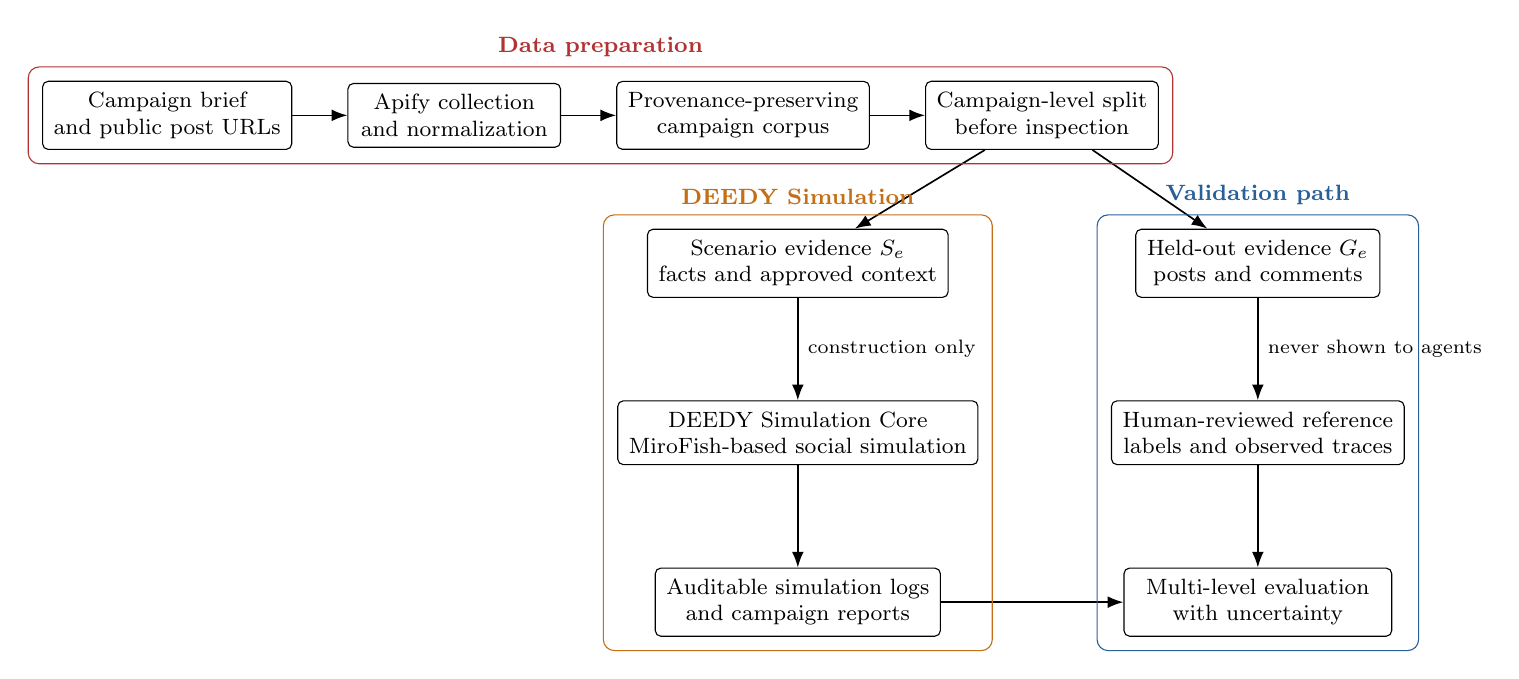
\begin{tikzpicture}[font=\footnotesize, node distance=5mm and 7mm]
        \node[deedybox, minimum width=27mm] (sources)
            {Campaign brief\\and public post URLs};
        \node[deedybox, minimum width=27mm, right=of sources] (collect)
            {Apify collection\\and normalization};
        \node[deedybox, minimum width=28mm, right=of collect] (freeze)
            {Provenance-preserving\\campaign corpus};
        \node[deedybox, minimum width=28mm, right=of freeze] (split)
            {Campaign-level split\\before inspection};

        \node[deedybox, minimum width=31mm, below left=10mm and -3mm of split]
            (scenario) {Scenario evidence $S_e$\\facts and approved context};
        \node[deedybox, minimum width=31mm, below right=10mm and -3mm of split]
            (holdout) {Held-out evidence $G_e$\\posts and comments};
        \node[deedybox, minimum width=34mm, below=13mm of scenario] (core)
            {DEEDY Simulation Core\\MiroFish-based social simulation};
        \node[deedybox, minimum width=34mm, below=13mm of holdout] (reference)
            {Human-reviewed reference\\labels and observed traces};
        \node[deedybox, minimum width=34mm, below=13mm of core] (outputs)
            {Auditable simulation logs\\and campaign reports};
        \node[deedybox, minimum width=34mm, below=13mm of reference] (evaluate)
            {Multi-level evaluation\\with uncertainty};

        \draw[deedyarrow] (sources) -- (collect);
        \draw[deedyarrow] (collect) -- (freeze);
        \draw[deedyarrow] (freeze) -- (split);
        \draw[deedyarrow] (split) -- (scenario);
        \draw[deedyarrow] (split) -- (holdout);
        \draw[deedyarrow] (scenario) -- node[right, font=\scriptsize]
            {construction only} (core);
        \draw[deedyarrow] (holdout) -- node[right, font=\scriptsize]
            {never shown to agents} (reference);
        \draw[deedyarrow] (core) -- (outputs);
        \draw[deedyarrow] (outputs) -- (evaluate);
        \draw[deedyarrow] (reference) -- (evaluate);

        \node[draw=deedyred, rounded corners=4pt,
            fit=(sources)(collect)(freeze)(split), inner sep=5pt,
            label={[text=deedyred,font=\bfseries\footnotesize]above:Data preparation}] {};
        \node[draw=deedyorange, rounded corners=4pt,
            fit=(scenario)(core)(outputs), inner sep=5pt,
            label={[text=deedyorange,font=\bfseries\footnotesize]above:DEEDY Simulation}] {};
        \node[draw=deedyblue, rounded corners=4pt,
            fit=(holdout)(reference)(evaluate), inner sep=5pt,
            label={[text=deedyblue,font=\bfseries\footnotesize]above:Validation path}] {};
    \end{tikzpicture}
    \caption{DEEDY application architecture. Campaign evidence is frozen and
    partitioned before simulation: only $S_e$ constructs the scenario, while
    $G_e$ remains hidden until the simulation logs and reports are evaluated.
    This is a data-partition and evaluation architecture, not a model
    training/test pipeline.}
    \label{fig:deedy-architecture}
\end{figure*}

\subsection{System Architecture Overview}

Figure~\ref{fig:deedy-architecture} organizes DEEDY into three layers. The
\emph{data layer} selects campaign posts, collects comments through Apify,
cleans, partitions, and annotates Thai campaign material. The \emph{core layer}
supplies the scenario summary to the \emph{DEEDY Simulation Core}, which uses
MiroFish to construct a GraphRAG-backed world and execute the hybrid
simulation layer. Its hybrid-ABM and dual-memory design is informed by the
ISAL-NLP architecture manuscript~\cite{marketfish2026architecture}. This layer
combines cognitive LLM agents with stochastic public agents, dual memory,
FYP or KOL seeding, network propagation, and an optional information-operations
stress test. The
\emph{validation layer} compares outputs with social posts and comments never
shown to the agents. Every derived artifact records a campaign identifier,
platform, post URL, provenance pointer, processing version, and experimental
split so that a score can be traced back to its evidence.

\subsection{Data Preparation Pipeline}

\subsubsection{Campaign Definition and Post Selection}

The input manifest \texttt{data/topic\_ref.json} defines one marketing campaign
per record through a campaign topic and a list of reference URLs. URLs may
refer to campaign posts, creator or influencer posts, news coverage, or public
community posts on Facebook, Instagram, and TikTok. Including more than the
brand's official account reduces the risk of measuring only an owned-audience
response. For an experimental release, the manifest is extended with a stable
campaign identifier, observation window, and source stratum. Each URL is
manually checked for campaign relevance and resolved to a canonical post before
collection. The sampling frame and inclusion rules are frozen before labels or
simulation outputs are inspected.

Campaign facts used to construct the simulated scenario are stored separately
from consumer reactions. The factual packet may include the campaign brief,
creative copy, product information, publication time, and dated public
reporting. It does not include the target comments later used for evaluation.
This distinction supports both retrospective campaign analysis and a stricter
prospective design in which only information available at campaign launch is
provided to the agents.

\subsubsection{Apify Comment Collection}
\label{sec:apify-collection}

DEEDY uses Apify Actors as the collection interface rather than a manually
maintained browser crawler. An Actor is a server-side program that accepts
structured input, executes as a recorded run, and writes results to an Apify
dataset accessible through the API or client libraries~\cite{apify2026actors}.
The implemented \texttt{apify\_crawler.py} detects the platform from each URL
and invokes \texttt{apify/facebook-comments-scraper},
\texttt{apify/instagram-comment-scraper}, or
\texttt{clockworks/tiktok-comments-scraper}. A platform adapter maps each
Actor's output into one common comment schema.

The collection unit is one social-media post. Under the revised protocol,
DEEDY launches an independent Actor query for every canonical post URL with a
requested limit of
\textbf{1,000 comments per post}. The limit is reset for each URL; it is not a
shared 1,000-comment budget for the campaign or topic. If a campaign contains
$m$ posts, the intended maximum is therefore
\begin{equation}
    N_{\max}=1{,}000m.
\end{equation}
The returned count may be lower when a post has fewer comments or when the
platform or Actor cannot expose every comment. Replies are configured
explicitly for each platform and are counted as separate records when returned.
Accordingly, ``1,000'' is a reproducible query cap, not a guarantee of 1,000
observations and not a claim of complete platform coverage.

\subsubsection{Normalization and Provenance}

Each returned item is validated and normalized to the fields
\texttt{topic}, \texttt{platform}, \texttt{post\_url},
\texttt{comment\_id}, anonymized \texttt{author}, \texttt{text},
\texttt{likes\_count}, \texttt{parent\_comment\_id}, and \texttt{timestamp}.
The parent identifier preserves reply structure when the Actor exposes it.
Missing values remain explicit rather than being inferred. Records without
comment text are excluded from content analysis but retained in run-level
quality-control counts when they represent Actor errors.

For reproducibility, a provenance manifest records the campaign and canonical
post identifiers, Actor identifier and version, complete run input, Apify run
and dataset identifiers, start and completion times, requested limit
(1,000), returned count, reply setting, error status, collection-code version,
and a checksum of the frozen raw export. Raw UTF-8 JSONL is immutable after a
successful run. Subsequent tables are derived from that snapshot and
de-duplicated first by platform comment identifier and then by normalized-text
similarity within a post. User names and platform identifiers are hashed or
removed before research analysis.

This design improves repeatability but does not turn the result into a random
sample. Search and post selection, platform ranking, deleted or moderated
comments, public visibility, geography, login state, and Actor behavior can all
affect what is returned. DEEDY therefore reports requested and observed counts
for every post and treats cross-platform comparisons as conditional on these
collection mechanisms.

\subsubsection{Thai-Aware Data Views}

The crawler preserves the Unicode comment text returned by each Actor in an
immutable JSONL view. The implemented
\texttt{convert\_comments\_to\_csv.py} then flattens nested post records into a
UTF-8-SIG table containing the campaign topic, comment, author, engagement,
platform, post, comment and parent identifiers, and timestamp. This second view
supports inspection and annotation without replacing the raw export.

DEEDY avoids aggressive text cleaning because emoji, Thai--English
code-mixing, orthographic repetition, hashtags, particles, negation, and
punctuation may carry campaign stance or affect. The analysis view standardizes
only encoding, line breaks, and whitespace; any additional transformation is
versioned and never overwrites the raw text. Thai tokenization is performed
only when a metric requires tokens, while character- and embedding-level
metrics are reported in parallel to reduce dependence on one segmentation
system.

\subsubsection{Evidence Split and Structured Weak Annotation}

For each campaign $e$, the collected evidence is partitioned before any model
summary is generated:
\begin{equation}
    D_e = S_e \;\dot\cup\; G_e,
\end{equation}
where $S_e$ is the scenario-construction set and $G_e$ is the held-out observed
reaction set. $S_e$ contains the campaign facts and context permitted at the
chosen simulation start time. $G_e$ contains comments and interactions that
the simulator must reproduce but never receives as memory. A post is assigned
wholly to one experimental role when post-level holdout is used; temporal
experiments instead apply a pre-registered timestamp cut. Comment identifiers,
quoted passages, and near duplicates cannot cross the boundary.

The frozen Apify records are passed to \texttt{llm\_prelabel.py} in bounded
batches. Three critique models independently assign a positive, neutral, or
negative label to each sampled comment and summarize campaign response. A
fourth model synthesizes their outputs into consensus sentiment labels, an
overall sentiment-direction analysis, recommended campaign next steps, and
possible business or operational changes. Exact sentiment counts are computed
from the consolidated comment-level labels rather than estimated from the
synthesis text. Additional evaluation labels for campaign stance, narrative,
purchase intent, and sarcasm are collected under the human-annotation protocol
rather than attributed to the current pre-labeling script.

These model outputs are \emph{weak pre-annotations}, not ground truth. Only a
summary derived from $S_e$ may enter MiroFish; labels or summaries derived from
$G_e$ are restricted to scoring and error analysis. Before the main experiment,
native Thai annotators review a frozen, source-stratified sample, adjudicate
disagreements, report Krippendorff's $\alpha$, and audit errors involving
sarcasm, code-mixing, indirect criticism, and platform source. This separation
prevents observed campaign reactions from leaking into agent memory.

\subsection{DEEDY Simulation Core}

Figure~\ref{fig:core-technology} makes the core execution path explicit. It
names the deployed component \emph{DEEDY Simulation Core}; MiroFish is the
underlying simulation engine. The hybrid-ABM and dual-memory architecture is
informed by the ISAL-NLP MarketFish manuscript~\cite{marketfish2026architecture}.
DEEDY adds the scenario packet, GraphRAG grounding, Thai actor attributes,
provenance, and the external holdout protocol described in this paper.

\begin{figure*}[t]
    \centering
    \resizebox{0.96\textwidth}{!}{%
    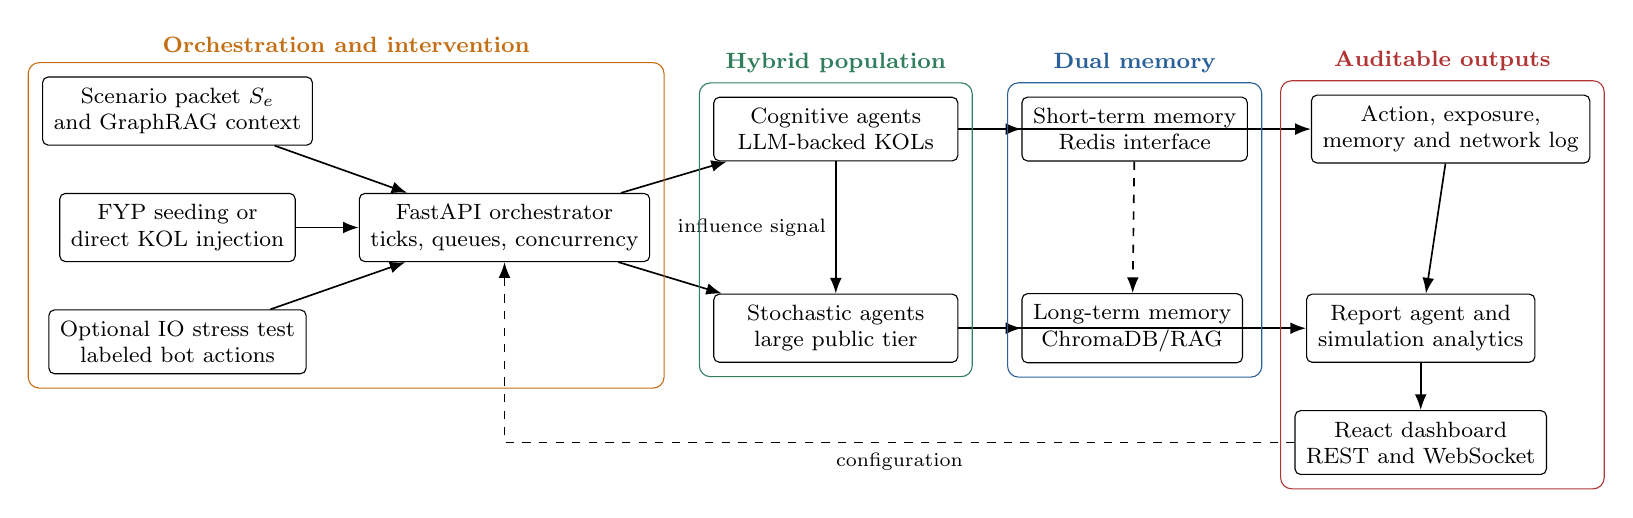
\begin{tikzpicture}[font=\footnotesize, node distance=6mm and 8mm]
        \node[deedybox, minimum width=29mm] (packet)
            {Scenario packet $S_e$\\and GraphRAG context};
        \node[deedybox, minimum width=29mm, below=of packet] (seed)
            {FYP seeding or\\direct KOL injection};
        \node[deedybox, minimum width=29mm, below=of seed] (io)
            {Optional IO stress test\\labeled bot actions};

        \node[deedybox, minimum width=32mm, right=8mm of seed] (orch)
            {FastAPI orchestrator\\ticks, queues, concurrency};

        \node[deedybox, minimum width=31mm, above right=4mm and 8mm of orch]
            (cognitive) {Cognitive agents\\LLM-backed KOLs};
        \node[deedybox, minimum width=31mm, below right=4mm and 8mm of orch]
            (math) {Stochastic agents\\large public tier};

        \node[deedybox, minimum width=28mm, right=8mm of cognitive] (redis)
            {Short-term memory\\Redis interface};
        \node[deedybox, minimum width=28mm, right=8mm of math] (chroma)
            {Long-term memory\\ChromaDB/RAG};

        \node[deedybox, minimum width=29mm, right=8mm of redis] (log)
            {Action, exposure,\\memory and network log};
        \node[deedybox, minimum width=29mm, right=8mm of chroma] (report)
            {Report agent and\\simulation analytics};
        \node[deedybox, minimum width=29mm, below=of report] (ui)
            {React dashboard\\REST and WebSocket};

        \draw[deedyarrow] (packet) -- (orch);
        \draw[deedyarrow] (seed) -- (orch);
        \draw[deedyarrow] (io) -- (orch);
        \draw[deedyarrow] (orch) -- (cognitive);
        \draw[deedyarrow] (orch) -- (math);
        \draw[deedyarrow] (cognitive) -- node[left, font=\scriptsize]
            {influence signal} (math);
        \draw[deedydashed] (cognitive) -- (redis);
        \draw[deedydashed] (math) -- (chroma);
        \draw[deedydashed] (redis) -- (chroma);
        \draw[deedyarrow] (cognitive) -- (log);
        \draw[deedyarrow] (math) -- (report);
        \draw[deedyarrow] (log) -- (report);
        \draw[deedyarrow] (report) -- (ui);
        \draw[deedydashed] (ui.west) -| node[pos=.25, below, font=\scriptsize]
            {configuration} (orch.south);

        \node[draw=deedyorange, rounded corners=4pt,
            fit=(packet)(seed)(io)(orch), inner sep=5pt,
            label={[text=deedyorange,font=\bfseries\footnotesize]above:Orchestration and intervention}] {};
        \node[draw=deedygreen, rounded corners=4pt,
            fit=(cognitive)(math), inner sep=5pt,
            label={[text=deedygreen,font=\bfseries\footnotesize]above:Hybrid population}] {};
        \node[draw=deedyblue, rounded corners=4pt,
            fit=(redis)(chroma), inner sep=5pt,
            label={[text=deedyblue,font=\bfseries\footnotesize]above:Dual memory}] {};
        \node[draw=deedyred, rounded corners=4pt,
            fit=(log)(report)(ui), inner sep=5pt,
            label={[text=deedyred,font=\bfseries\footnotesize]above:Auditable outputs}] {};
    \end{tikzpicture}%
    }
    \caption{DEEDY Simulation Core architecture. The core is MiroFish-based and
    its hybrid-ABM and dual-memory design is informed by the ISAL-NLP MarketFish
    manuscript~\cite{marketfish2026architecture}. The orchestrator combines
    configurable exposure and intervention with a hybrid cognitive--stochastic
    population; agents use short- and long-term memory, and their traces feed
    reporting and the live application. Solid arrows denote the main
    execution/data path; dashed arrows denote memory or configuration access.}
    \label{fig:core-technology}
\end{figure*}

\subsubsection{Reality Seed, GraphRAG, and Dual Memory}

The scenario packet contains the campaign brief, creative message, dated
factual claims, named entities, brands, products, creators, and source-level
provenance from $S_e$.
MiroFish extracts an ontology and entity relations, then injects individual and
collective memories into its graph retrieval layer~\cite{mirofish2026}. A
retrieved memory attached to an agent action includes its supporting node or
source identifier. Unsupported details generated during graph construction are
marked as model assumptions and are not silently promoted to facts.

The ISAL component design adds two timescales of per-agent memory
~\cite{marketfish2026architecture}. A short-term
store holds exposures, private-state updates, and interactions within the
active simulation window; a persistent ChromaDB store holds vectorized prior
and reflected memories retrieved across rounds. This division reduces the
``cold start'' behavior of blank-slate agents without exposing them to the
evaluation set: only material from $S_e$, together with events generated inside
the simulation, may enter either store. Retrieval records the memory identifier,
source class, similarity score, and simulated timestamp. The research
prototype exposes a Redis-compatible short-term interface but currently uses
an in-process substitute, so Redis latency and durability are not claimed as
evaluated results.

\subsubsection{Actor and Environment Construction}

Actors represent campaign-relevant audience roles justified by $S_e$, such as
existing customers, prospective customers, creator followers, brand advocates,
skeptics, journalists, community members, and bystanders. A profile separates
evidence-backed attributes from sampled attributes. The Thai adaptation adds
language register, Thai--English mixing rate, region or dialect only when
supported, politeness strategy, typical message length, activity rate,
campaign-interest prior, interests, and uncertainty. Demographic attributes
are not inferred from a single message. Population weights and network links
are sampled from documented priors and varied during sensitivity analysis
rather than presented as known facts.

The environment specifies platforms, action space, time step, feed capacity,
and recommendation mechanism. OASIS supplies posting, replying, reposting,
following, and browsing behavior with dynamic social and content state
~\cite{yang2024oasis}. DEEDY additionally records each exposure before an
action. This makes it possible to distinguish ``the agent never saw the
message'' from ``the agent saw and rejected the message,'' a necessary
distinction for interpreting diffusion failure.

\subsubsection{Hybrid Cognitive--Stochastic Population}

Directly invoking an LLM for every decision limits population size, increases
cost, and makes a viral exposure burst vulnerable to rate limits. DEEDY
therefore integrates the ISAL manuscript's hybrid ABM design
~\cite{marketfish2026architecture}. Let
$\mathcal{A}=\mathcal{C}\,\dot\cup\,\mathcal{M}$ be the agent population, where
$\mathcal{C}$ contains cognitive agents and $\mathcal{M}$ contains stochastic
mathematical agents. The cognitive tier is a small, configurable share of the
population---5\% in the prototype configuration, rather than a universal
constant---and is assigned to influential or analytically important roles.
These agents retrieve memory, update private stance, generate context-aware
Thai language, and choose among platform actions. The remaining public agents
retain a profile, prior bias, network position, and exposure history, but use a
lightweight probabilistic response rule.

For an exposed mathematical agent $i$ at round $t$, the probability of taking
a visible action rather than abstaining is represented as
\begin{equation}
    \Pr(a_{i,t}\neq\varnothing)=\sigma\!\left(
    \beta_0 + \beta_b b_i + \boldsymbol{\beta}_d^{\top}\mathbf{d}_i
    + \beta_s s_{t-1} + \beta_x x_{i,t}\right),
    \label{eq:hybrid-response}
\end{equation}
where $\sigma$ is the logistic function, $b_i$ is the agent's pre-campaign
bias, $\mathbf{d}_i$ contains documented population attributes, $s_{t-1}$ is
the preceding visible sentiment trend, and $x_{i,t}$ contains exposure and
neighbor signals. A second categorical draw selects like, share, comment, or
silence. All coefficients, tier ratios, and random seeds are versioned per run.
The model does not assume that public opinion is determined by KOL output:
tier-specific results are logged, and sensitivity analysis varies both the
cognitive share and $\beta_s$ to reveal artificial herding.

\subsubsection{Algorithmic Seeding and Network Propagation}

The initial exposure mechanism represents discovery outside a follower graph.
Under FYP seeding, round 1 places the campaign in the observation queues of a
configured sample of eligible agents. Under KOL injection, the same campaign is
delivered first to selected high-influence cognitive agents. Later rounds
propagate shares over a configurable small-world or observed interaction graph.
The exposure probability is
\begin{equation}
    p^{\mathrm{see}}_{i,t}=\operatorname{clip}_{[0,1]}\!\left[
    \alpha f_{i,t}+(1-\alpha)
    \sum_{j\in\mathcal{N}(i)}w_{j,i}
    I^{\mathrm{share}}_{j,t-1}\right],
    \label{eq:algorithmic-exposure}
\end{equation}
where $f_{i,t}$ is algorithmic eligibility or targeting, $\mathcal{N}(i)$ is
the neighbor set, $w_{j,i}$ is directed influence, and
$I^{\mathrm{share}}_{j,t-1}$ indicates a share in the previous round. When the
prior wave's engagement exceeds a pre-registered threshold $\tau$, the FYP mechanism may
open a secondary wave to unreached strata. The seed size, $\alpha$, $\tau$,
edge construction, and eligibility policy are experimental assumptions, not
reconstructions of a platform's proprietary recommender. Chronological,
popularity, and interest-based policies remain comparison conditions.

\subsubsection{Thai Context in Perception and Action}

At each round, an actor retrieves relevant graph memory, observes a bounded
feed, updates a private state, and chooses an action or abstention. Prompts
require natural Thai consistent with the actor's register without demanding
caricatured dialect. They preserve uncertainty, allow silence, and prohibit
fabricated quotations or demographic claims. Conversation context is included
for reply generation because Thai stance and sarcasm may depend on an earlier
turn~\cite{hazarika2018cascade}. The language model is configurable: a
Thai-optimized model such as Typhoon 2 can be compared with multilingual
models under identical action rules rather than assuming that any model is
superior. In the executable pilot, the OpenAI-compatible OpenRouter endpoint
was configured with pinned \texttt{deepseek/deepseek-v4-flash-0731} and
\texttt{qwen/qwen3-8b} revisions. Neither is treated as a Thai-specialized
control; their comparison tests the configured model path and cost--quality
trade-off, while the native-Thai model comparison remains future work.

\subsubsection{Information-Operations Stress Testing}

The optional information-operations (IO) module assigns a pre-registered share
of mathematical agents to coordinated positive promotion or negative attack.
Their injected actions are explicitly labeled and kept separate from organic
responses, allowing the analyst to measure changes in reach, sentiment,
polarization, and cross-group adoption as the IO rate varies. This module is a
counterfactual robustness test, not a detector of real accounts and not a claim
that authentic Thai users follow bot behavior. It is disabled in the primary
correspondence experiment unless IO prevalence is itself the registered factor.

\subsubsection{Simulation Outputs and Application Layer}

An asynchronous FastAPI orchestration service accepts simulation configuration
through REST, bounds concurrent LLM requests, and publishes tick, action,
network, and aggregate updates to the React application through WebSockets.
This permits a live matrix feed without making UI delivery part of the agent's
decision rule. The core also returns a machine-readable simulation log and a
human-readable campaign report. The
log contains agent state version, exposure set, retrieved evidence, selected
action, generated content, parent action, timestamp, and token/model settings.
The report summarizes dominant and minority narratives, sentiment and stance
trajectories, campaign reach, engagement mix, influential nodes, propagation
paths, disagreement, and unsupported claims. Live sentiment timelines and
reach distinguish exposed-and-engaged agents from exposed-but-silent agents;
unreached agents remain a third category. The report also exposes uncertainty
across runs and separates cognitive, mathematical, and injected IO activity.

The application allows a marketer or analyst to select a campaign, inspect the
scenario packet and graph, configure actor count, hybrid-tier ratio, seed
policy, feed policy, and IO mode, run a baseline or a counterfactual campaign
message, compare it with held-out
observations, and drill down from an aggregate chart to the simulated posts
and evidence that produced it. Counterfactual reports compare conditions
inside the model; they are not presented as causal effects in the real Thai
consumer population.

\section{Experimental Design}

\subsection{Research Questions}

The evaluation is organized around four questions:
\begin{itemize}
    \item \textbf{RQ1 (Content):} Does DEEDY reproduce the sentiment, stance,
    narrative, and linguistic characteristics of held-out Thai reactions?
    \item \textbf{RQ2 (Population):} Does graph grounding and Thai adaptation
    improve aggregate correspondence without collapsing response diversity?
    \item \textbf{RQ3 (Dynamics):} Does the simulated interaction process match
    observed cascade size, shape, timing, and network structure?
    \item \textbf{RQ4 (Application):} Are campaign reports traceable, stable
    across repeated runs, and useful to Thai marketing analysts without
    overstating certainty?
\end{itemize}

\subsection{Dataset and Splitting Protocol}

The initial study will select campaigns with at least one usable factual
scenario packet and multiple public campaign-related posts. Before simulation,
the protocol freezes the required minimum returned-comment count, eligible
platforms, post-source strata, and missing-data rules. Apify then receives a
separate query for each post with a 1,000-comment limit as described in
Section~\ref{sec:apify-collection}. Posts returning fewer records are retained
when they satisfy the pre-registered minimum; the dataset never pads a short
thread by duplicating comments or borrowing another post's quota.

The unit of generalization is a \emph{campaign}, not an individual post or
comment. Prompt and model selection use development campaigns, and final
scores are reported on untouched test campaigns. Within a campaign, $S_e$ and
$G_e$ are separated either by a pre-registered timestamp or by whole post so
that a reaction thread cannot leak into both construction and evaluation.
Actor run inputs, query dates, returned counts, source strata, and split
assignments are frozen before weak annotation. This design supports
source-balanced analysis, temporal-drift checks, and sensitivity to
platform-specific public visibility.

Weak labels are independently reviewed by at least three native Thai
annotators using a codebook for three-way sentiment, campaign-specific stance,
sarcasm, and narrative membership. Annotators see necessary conversational
context but not whether a post is real or simulated during quality comparison.
Majority/adjudicated labels form the reference set, and Krippendorff's
$\alpha$ is reported for each task. User identifiers are hashed and quoted
examples are paraphrased unless publication is ethically justified.

\begin{table*}[t]
\caption{Planned experiments. Each condition is run with the same campaign
split, agent budget, round budget, and ten random seeds unless that factor is
varied.}
\label{tab:experiments}
\centering
\footnotesize
\begin{tabular}{@{}p{0.16\textwidth}p{0.31\textwidth}p{0.43\textwidth}@{}}
\toprule
Experiment & Conditions & Primary purpose \\
\midrule
Exp. 1: Grounding & DEEDY seed-only; ungrounded LLM agents; deliberately leaky
all-source upper bound & Test whether held-out correspondence comes from the
scenario pipeline rather than parametric knowledge or target leakage. \\
Exp. 2: Thai adaptation & Full Thai adaptation; translated/unadapted MiroFish;
normalization without context features & Measure sentiment/stance distance,
narrative coverage, Thai quality, sarcasm, code-mixing, and diversity. \\
Exp. 3: Core model & DeepSeek V4 Flash 0731; Qwen3 8B; simple non-generative
ABM baseline in the pilot, followed by a matched Thai-specialized comparison
in the confirmatory study & Separate the contribution of the language model
from the graph, population, and platform mechanisms. \\
Exp. 4: Social mechanism & Chronological, popularity, and interest feeds;
observed versus random network; multiple population sizes & Test cascade,
polarization, herding, and sensitivity to platform assumptions. \\
Exp. 5: Application & Baseline campaign versus one pre-registered
message-framing
counterfactual; report with versus without uncertainty/evidence links & Assess
traceability, analyst usefulness, and whether presentation changes trust. \\
\bottomrule
\end{tabular}
\end{table*}

\subsection{Metrics}

\subsubsection{Content and Population Correspondence}

Let $P_G^y$ and $P_S^y$ be observed and simulated distributions for label
$y\in\{\text{sentiment},\text{stance},\text{narrative}\}$. Distributional
correspondence is measured with Jensen--Shannon distance:
\begin{equation}
 d_{\mathrm{JS}}(P_G^y,P_S^y)=
 \sqrt{\tfrac{1}{2}D_{\mathrm{KL}}(P_G^y\Vert M)+
 \tfrac{1}{2}D_{\mathrm{KL}}(P_S^y\Vert M)},
\end{equation}
where $M=(P_G^y+P_S^y)/2$. Lower is better and the square-root form is bounded.
Macro-F1 is also reported when simulated posts are matched to a conditioned
stimulus or stance target.

Narrative correspondence is measured in two ways. First, Thai annotators map
posts to a campaign-specific narrative codebook and we compare coverage and
prevalence. Second, multilingual BERTScore measures semantic similarity between
generated and observed response sets~\cite{zhang2020bertscore}. Embedding-based
scores are treated as complementary because semantic proximity need not imply
the same stance. Diversity is reported using Distinct-1/2, Self-BLEU, unique
narrative count, lexical entropy, length distribution, and pairwise embedding
distance. High correspondence accompanied by diversity collapse is considered
a failure.

Polarization is measured from the stance distribution and interaction graph.
We report normalized stance entropy, between-group versus within-group
interaction, and modularity after fixing the community-detection procedure.
Population statistics are computed per run and then aggregated across
campaigns, so campaigns with many selected posts do not automatically dominate
the result.

\subsubsection{Temporal and Network Correspondence}

For trace-enriched campaigns, cumulative activity curves are aligned to the
campaign-post publication time. We report normalized root-mean-square error
(NRMSE) and dynamic time
warping distance, together with cascade scale, maximum depth, maximum breadth,
structural virality, time to 50\% of final activity, and peak-time error. OASIS
uses scale, depth, breadth, and propagation-curve error in its own validation
~\cite{yang2024oasis}; DEEDY adds exposure-conditioned action rates and Thai
content labels.

Observed and simulated interaction graphs are compared by degree and cascade-
size distributions using the two-sample Kolmogorov--Smirnov statistic, plus
clustering coefficient, reciprocity, assortativity, modularity, and the share
of cross-stance replies. These metrics are omitted, rather than imputed, when
the source platform does not expose the required trace.

\subsubsection{Thai Quality and Report Evaluation}

Native Thai raters score blinded real and simulated posts on a five-point scale
for naturalness, contextual coherence, stance consistency, pragmatic and
cultural appropriateness, and persona consistency. Sarcasm precision, recall,
and F1 are evaluated separately. Report claims are scored for evidence
traceability: the proportion of factual claims linked to scenario evidence or
simulation events, unsupported-claim rate, contradiction rate, and coverage of
minority narratives.

An LLM judge may assist high-volume screening, but cannot be the sole quality
measure. Pair order is swapped, output identity is hidden, the judge must cite
the supplied evidence before scoring, and its agreement with Thai raters is
reported. These controls address known position bias in LLM-as-a-judge
evaluation~\cite{shi2024judging}.

\subsection{Execution and Statistical Analysis}

All stochastic conditions use ten seeds initially; a power analysis on pilot
variance determines the final number. Model name and revision, prompts,
temperature, top-$p$, agent count, network seed, recommendation parameters,
round count, stopping rule, and token cost are frozen before the test set is
opened. We report medians and 95\% bootstrap confidence intervals across
campaigns. Paired conditions use a campaign-level permutation test or Wilcoxon
signed-rank test with Holm correction. Effect sizes accompany $p$-values.

The OpenRouter pilot fixes temperature at 0.8, the completion ceiling at 2,200
tokens, reasoning mode off, concurrency at 12, and ten requested seeds. Each
call asks for 12 structured synthetic Thai reactions. Five campaigns, five
prompt conditions, two models, and ten seeds yield 500 unique calls. The
seed-only condition is reused when expanding Experiments~1--3, producing 750
metric rows without making duplicate provider requests. Model-returned
sentiment labels are diagnostic self-reports rather than independent
annotations.

The main comparison is the full DEEDY pipeline versus translated/unadapted
MiroFish. Component ablations remove graph retrieval, Thai context features,
thread context, or observed population weights one at a time. The deliberately
leaky condition in Table~\ref{tab:experiments} is never a valid system result;
it is a diagnostic ceiling showing how much apparent performance can be gained
by exposing held-out reactions.

\subsection{Acceptance Criteria for the Application}

Before results are observed, the study will set minimum criteria: (i) full
pipeline completion and provenance for every scored run; (ii) statistically
lower sentiment/stance Jensen--Shannon distance than the unadapted baseline;
(iii) no significant diversity collapse relative to held-out posts; (iv) Thai
quality above the midpoint with acceptable annotator agreement; (v) report
unsupported-claim rate below a pre-registered threshold; and (vi), for
trace-enriched campaigns, improvement on at least two cascade metrics without
material degradation on the others. Failure remains a reportable result and
defines the application's operating boundary.

\section{Automated Pilot Results}
\label{sec:pilot-results}

\subsection{Execution Scope and Reproducibility}

An automated pilot was executed on 28 August 2026 to verify that the revised
MiroFish application, non-generative ABM baseline, parameter sweep, provenance
capture, and report path run end to end. The Docker image was built locally
after adding the missing FastAPI runtime dependencies and switching the launch
path to the current \texttt{frontend-v2} application. With cloud credentials
absent during the first run, the web shell remained available while LLM- and
Zep-dependent operations remained disabled. The backend health endpoint and
frontend both returned HTTP 200 during the recorded run. A second Dockerized
run on 29 August 2026 (Bangkok time) exercised the OpenRouter LLM path for
Experiments~1--3. On 30 August, a further leakage-guarded cognitive-agent panel
exercised the LLM path for Experiments~4--5. Zep-dependent graph-memory
operations were not required for these bounded prompt-level pilots.

The pilot used seeds 1--10, 12 rounds, requested mean degree 6, and populations
of 200, 500, and 1,000. Experiment~4 comprised 900 runs
($5$ campaigns $\times 3$ feed policies $\times 2$ network assumptions
$\times 3$ population sizes $\times 10$ seeds). The automated portion of
Experiment~5 added 100 runs ($5$ campaigns $\times 2$ message conditions
$\times 10$ seeds) at $N=500$. Experiments~1--3 added 500 unique OpenRouter
calls and 750 expanded metric rows. The Experiment~4--5 panel added 800 calls:
600 for the $5\times3\times2\times10\times2$
campaign--feed--network--seed--model design and 200 for the
$5\times2\times10\times2$ baseline/clarity--seed--model design. Each call
requested eight cognitive-agent records, yielding 6,400 schema-valid reactions.
Input SHA-256 hashes, parameters, run-level
records, aggregate tables, smoke-test responses, provider pricing, and
interpretation limits are stored in \texttt{MiroFish\_App/result/manifest.json},
\texttt{llm\_exp123\_manifest.json}, \texttt{llm\_exp45\_manifest.json}, and
the accompanying machine-readable
files. No authentic comment text, author identifier, or post URL was placed in
the result bundle or sent to OpenRouter.

Table~\ref{tab:pilot-coverage} distinguishes executed work from the evaluation
still required for the paper's main claims. In particular, this pilot does not
substitute model self-labels or character ratios for independent held-out
labels, native-Thai ratings, or analyst judgments.

\begin{table*}[t]
\caption{Coverage of the planned experiments in the automated pilot.}
\label{tab:pilot-coverage}
\centering
\footnotesize
\begin{tabular}{@{}p{0.16\textwidth}p{0.74\textwidth}@{}}
\toprule
Experiment & Pilot status \\
\midrule
Exp. 1: Grounding & Seed-only, ungrounded, and deliberately leaky prompt
conditions were run for two models; independent held-out scenario packets
remain unavailable. \\
Exp. 2: Thai adaptation & Three prompt-level conditions were run for two
models; native-Thai reference ratings remain unavailable. \\
Exp. 3: Core model & DeepSeek V4 Flash 0731, Qwen3 8B, and the simple
non-generative ABM were run; the Thai-specialized and full hybrid-tier
comparison remains pending. \\
Exp. 4: Social mechanism & The full non-generative feed, network-assumption,
and population-size sweep and a two-model prompt-conditioned cognitive-agent
panel were run with ten seeds; a full LLM/OASIS reply trajectory remains pending. \\
Exp. 5: Application & Docker health, result provenance, a paired internal ABM
counterfactual, and a paired two-model LLM clarity-frame panel were run;
analyst usefulness and presentation effects were not rated. \\
\bottomrule
\end{tabular}
\end{table*}

\subsection{Dataset and Trace Audit}

The supplied aggregate file and crawl contained five campaigns and exactly
5,000 comments from 33 posts. Each campaign contributed 1,000 comments. The
campaign-specific unique-author counts ranged from 946 to 981. However, all
5,000 records had a null \texttt{parent\_comment\_id}. An observed reply graph
and empirical cascade tree therefore could not be reconstructed. In accordance
with the missing-trace rule in the experimental design, the pilot does not
report observed cascade correspondence. For the mechanism sensitivity test,
the planned observed-network condition was replaced by an explicitly labeled
\emph{post-affiliation proxy}: agents sampled from the same source-post stratum
received local ties. Its comparator was a random graph with the same number of
edges. Neither graph should be described as an observed Thai interaction
network.

The sentiment distribution used to initialize each campaign was the summary
over all collected comments. Consequently, the Jensen--Shannon distance in this
section measures drift from a calibration target, not accuracy on held-out
reactions. This circular calibration would be invalid as evidence for RQ1 or
RQ2; it is retained only to diagnose whether the social mechanisms destabilize
the supplied aggregate proportions.

\subsection{OpenRouter LLM Diagnostics: Experiments 1--3}

All 500 provider calls completed. DeepSeek returned 2,983 of 3,000 requested
reactions; Qwen returned 3,000 of 3,000. Across all five prompt conditions,
DeepSeek's 250 calls averaged 35.51 seconds and cost \$0.0276, whereas Qwen's
250 calls averaged 15.17 seconds and cost \$0.1109. The complete run cost
\$0.1386. Thus, Qwen was faster in this execution, but DeepSeek was about four
times less expensive. These totals depend on the provider route, token counts,
and prices recorded in the manifest and are not universal model benchmarks.

Table~\ref{tab:pilot-exp12} reports sentiment JSD and a character-level Thai
ratio. In Experiment~1, the paired seed-only-minus-ungrounded JSD was $-0.0063$
for DeepSeek (empirical 2.5--97.5 percentile interval $-0.1483$ to $0.1756$)
and $0.0471$ for Qwen ($-0.3313$ to $0.3484$). Both intervals span zero. The
leaky condition had lower mean JSD, but this expected result is invalid as
system performance because target aggregates were supplied to its prompt.

\begin{table*}[t]
\caption{Experiments~1--2 OpenRouter diagnostics. Each cell averages five
campaigns and ten seeds. Sentiment JSD is distance from an all-comment
calibration target, not held-out accuracy; the leaky row is invalid by design.}
\label{tab:pilot-exp12}
\centering
\footnotesize
\begin{tabular}{@{}llrrrr@{}}
\toprule
Experiment & Condition & DeepSeek JSD & Qwen JSD & DeepSeek Thai ratio & Qwen Thai ratio \\
\midrule
Exp. 1 & Seed only & 0.2572 & 0.2859 & 0.9822 & 0.9922 \\
Exp. 1 & Ungrounded & 0.2635 & 0.2388 & 0.9734 & 0.9561 \\
Exp. 1 & Leaky invalid bound & 0.2031 & 0.1966 & 0.9894 & 0.9927 \\
Exp. 2 & Thai-context prompt & 0.2572 & 0.2859 & 0.9822 & 0.9922 \\
Exp. 2 & Translated/unadapted & 0.2604 & 0.2523 & 0.9978 & 0.9611 \\
Exp. 2 & Normalization, no context & 0.2460 & 0.2548 & 0.9797 & 0.9736 \\
\bottomrule
\end{tabular}
\end{table*}

For Experiment~2, Thai-context-minus-translated JSD was $-0.0032$ for
DeepSeek ($-0.1444$ to $0.1344$) and $0.0337$ for Qwen ($-0.1988$ to $0.3302$).
The Thai-context-minus-normalization intervals also spanned zero. Thai-context
responses were longer than normalization-only responses for 49 of 50 DeepSeek
pairs and all 50 Qwen pairs, but had lower character-bigram diversity on
average. These prompt proxies therefore do not establish that Thai adaptation
improved quality. Thai-character ratios of 0.956--0.998 show script use, not
naturalness, cultural appropriateness, sarcasm fidelity, or code-mixing quality.

Table~\ref{tab:pilot-exp3} compares the shared seed-only condition with the
uniform non-generative baseline. DeepSeek-minus-Qwen JSD was $-0.0287$
($-0.3592$ to $0.2179$). DeepSeek-minus-ABM was $-0.0207$ ($-0.2341$ to
$0.1955$), and Qwen-minus-ABM was $0.0081$ ($-0.3765$ to $0.4340$). All
intervals span zero, so this pilot establishes no fidelity advantage for an
LLM tier or for either LLM. Qwen produced every requested schema item; the
DeepSeek seed-only rows were 0.9833 schema-valid and contained no exact
duplicates. Blinded native-Thai scoring and independent campaign holdouts are
still required.

\begin{table*}[t]
\caption{Experiment~3 core-model diagnostic over five campaigns and ten
seeds. Cost is mean provider cost per campaign-seed row. The ABM emits states,
not language.}
\label{tab:pilot-exp3}
\centering
\footnotesize
\begin{tabular}{@{}lrrrrr@{}}
\toprule
Condition & Sentiment JSD & Thai ratio & Valid share & Latency (s) & Cost/run \\
\midrule
DeepSeek V4 Flash 0731 & 0.2572 & 0.9822 & 0.9833 & 31.49 & \$0.000116 \\
Qwen3 8B & 0.2859 & 0.9922 & 1.0000 & 16.53 & \$0.000476 \\
Uniform non-generative ABM & 0.2779 & -- & 1.0000 & 0.00 & \$0.000000 \\
\bottomrule
\end{tabular}
\end{table*}

\subsection{Social-Mechanism Sensitivity}

Table~\ref{tab:pilot-exp4} reports the $N=500$ slice, averaging five campaigns
and ten seeds (50 runs per row). Results were strongly sensitive to the assumed
graph. The edge-matched random network produced mean action rates of
0.968--0.970 and reach of 0.997, whereas the post-affiliation proxy produced
action rates of 0.400--0.402 and reach of 0.461--0.463. This difference is a
property of the simulated propagation paths and is not an estimate of a
platform effect. Population-size sensitivity was smaller within each topology:
across the full sweep, mean action rates ranged from 0.965 to 0.970 for the
random graph and from 0.400 to 0.419 for the post-affiliation proxy.

The chronological feed had the lowest calibration drift at $N=500$
($d_{\mathrm{JS}}=0.077$ on the random graph and 0.082 on the proxy), followed
by the interest feed (0.102 and 0.097) and popularity feed (0.120 and 0.115).
Popularity also produced lower polarization in the random-graph condition.
These are descriptive sensitivity results from the non-generative rule set;
they do not establish that a real chronological feed is more accurate or less
polarizing.

\begin{table*}[t]
\caption{Experiment~4 automated pilot at $N=500$. Entries are means over five
campaigns and ten seeds. JSD is distance from the all-comment calibration
distribution, not held-out accuracy.}
\label{tab:pilot-exp4}
\centering
\footnotesize
\begin{tabular}{@{}llrrrrr@{}}
\toprule
Feed & Network assumption & Action rate & Reach & JSD & Polarization & Largest cascade \\
\midrule
Chronological & Matched random & 0.968 & 0.997 & 0.077 & 0.172 & 0.251 \\
Interest & Matched random & 0.970 & 0.997 & 0.102 & 0.138 & 0.224 \\
Popularity & Matched random & 0.968 & 0.997 & 0.120 & 0.126 & 0.239 \\
Chronological & Post-affiliation proxy & 0.402 & 0.463 & 0.082 & 0.169 & 0.159 \\
Interest & Post-affiliation proxy & 0.400 & 0.463 & 0.097 & 0.163 & 0.161 \\
Popularity & Post-affiliation proxy & 0.400 & 0.461 & 0.115 & 0.164 & 0.159 \\
\bottomrule
\end{tabular}
\end{table*}

\subsection{Leakage-Guarded LLM Cognitive-Agent Panel: Experiments 4--5}

The original Experiment~4--5 pilot above is a non-generative ABM. To inspect
LLM-generated actions, reactions, and stated reasons without leaking the
answer, we ran an additional prompt-conditioned cognitive-agent panel. Before
generation, each model received only one frozen campaign packet, one mechanism
condition, and eight Thai audience personas. It did not receive authentic
comments, the sentiment summary, or a summary derived from those comments.
Each returned record contains an action (like, share, comment, reply, or
silence), Thai reaction text, sentiment, stance, narrative label, confidence,
and a short \emph{rationale summary}. The latter is an auditable stated
explanation, not private chain-of-thought. Only after all 800 calls completed
did the scorer read the supplied
\texttt{campaign\_sentiment\_summary.csv} and compute
distance from its aggregate distributions.

Table~\ref{tab:llm-exp45-scenarios} records the scenario facts visible to the
agents and the all-comment target used only afterward for scoring. Parameter
Gelato was framed as a premium six-flavour launch at Siam Paragon; KFC Bucket
Ware as a limited reusable container redeemable for THB~99 after a THB~299
qualifying purchase; MK Buffet as a THB~299 net, 33-item offer with four
refillable seafood items and THB~59/129 upgrades; Top Charoen as a
walk/run-and-redeem eyewear campaign; and Thai Chuai Thai Plus as a 60/40
government co-payment through Paotang G-Wallet. The packets retained explicit
uncertainties concerning price or serving size, dates, eligibility,
participating locations, stock, entitlements, and extra charges rather than
inventing missing facts.

\begin{table*}[t]
\caption{Frozen Experiment~4--5 campaign packets and scoring-only targets.
Targets are negative/neutral/positive shares from the supplied all-comment
summary; none was included in an LLM prompt.}
\label{tab:llm-exp45-scenarios}
\centering
\scriptsize
\begin{tabular}{@{}p{0.16\textwidth}p{0.56\textwidth}p{0.18\textwidth}@{}}
\toprule
Campaign & Scenario facts supplied to the agents & Scoring target (neg./neu./pos.) \\
\midrule
Parameter Gelato & Premium gelato launch, Siam Paragon G floor, six curated
flavours; price, serving size, and availability left uncertain. & 0.362 / 0.476 / 0.162 \\
KFC Bucket Ware & Limited reusable container; THB~299 qualifying purchase plus
THB~99 redemption; dates, branches, and stock conditional. & 0.049 / 0.309 / 0.642 \\
MK Buffet & THB~299 net, 33 items and four refillable seafood items; optional
THB~59 and THB~129 upgrades; branch availability conditional. & 0.136 / 0.444 / 0.420 \\
Walk/Run for Glasses (Top Charoen) & Choose a distance, record the activity,
then redeem eligible eyewear; tracking, frame/lens entitlement, charges, stock,
and fulfilment left conditional. & 0.050 / 0.700 / 0.250 \\
Thai Chuai Thai Plus & Government 60/40 co-payment through Paotang G-Wallet;
eligibility, registration window, allowance, merchants, and exclusions follow
official rules. & 0.175 / 0.275 / 0.550 \\
\bottomrule
\end{tabular}
\end{table*}

Experiment~4 crossed chronological, interest, and popularity feed descriptions
with a matched-random or post-affiliation-proxy network description. It
produced 600 calls (50 campaign-seed runs per row) and 4,800 agent records.
Table~\ref{tab:llm-exp4} shows that the best aggregate correspondence was
DeepSeek with the chronological/matched-random prompt
($d_{\mathrm{JS}}=0.2995$). Across conditions, DeepSeek JSD ranged from 0.2995
to 0.3233 and Qwen from 0.3274 to 0.3432. Feed and network wording therefore
changed the prompt-level outputs only modestly in this panel. Generated agents
also under-produced negative reactions: mean negative share never exceeded
0.0225 although the campaign targets ranged from 0.049 to 0.362. This mismatch
is especially material for Parameter Gelato.

\begin{table*}[t]
\caption{Experiment~4 LLM cognitive-agent diagnostic. Each row averages five
campaigns and ten seeds. MR is matched random; PA is the post-affiliation
proxy. Visible action excludes silence.}
\label{tab:llm-exp4}
\centering
\scriptsize
\begin{tabular}{@{}llrrrrrrr@{}}
\toprule
Model & Feed/network & Runs & JSD & Visible action & Positive & Neutral & Negative \\
\midrule
DeepSeek & Chronological/MR & 50 & 0.2995 & 0.7825 & 0.4100 & 0.5700 & 0.0200 \\
DeepSeek & Chronological/PA & 50 & 0.3211 & 0.7800 & 0.3875 & 0.6050 & 0.0075 \\
DeepSeek & Interest/MR & 50 & 0.3159 & 0.7675 & 0.3975 & 0.5800 & 0.0225 \\
DeepSeek & Interest/PA & 50 & 0.3154 & 0.7750 & 0.3925 & 0.5925 & 0.0150 \\
DeepSeek & Popularity/MR & 50 & 0.3051 & 0.7825 & 0.4100 & 0.5825 & 0.0075 \\
DeepSeek & Popularity/PA & 50 & 0.3233 & 0.7600 & 0.3825 & 0.6100 & 0.0075 \\
Qwen & Chronological/MR & 50 & 0.3291 & 0.7450 & 0.3575 & 0.6400 & 0.0025 \\
Qwen & Chronological/PA & 50 & 0.3277 & 0.7450 & 0.3450 & 0.6500 & 0.0050 \\
Qwen & Interest/MR & 50 & 0.3389 & 0.7400 & 0.3375 & 0.6625 & 0.0000 \\
Qwen & Interest/PA & 50 & 0.3432 & 0.7400 & 0.3250 & 0.6725 & 0.0025 \\
Qwen & Popularity/MR & 50 & 0.3274 & 0.7475 & 0.3575 & 0.6425 & 0.0000 \\
Qwen & Popularity/PA & 50 & 0.3431 & 0.7525 & 0.3450 & 0.6550 & 0.0000 \\
\bottomrule
\end{tabular}
\end{table*}

For the generative Experiment~5 diagnostic, the interest/PA mechanism was held
fixed and each campaign-seed-model combination received either its baseline
packet or a clarity frame that made conditions and uncertainties more explicit.
The 200 calls yielded 1,600 agent records. As Table~\ref{tab:llm-exp5} shows,
clarity improved DeepSeek's mean JSD by 0.0074 but worsened Qwen's by 0.0015.
Across all 100 matched model--campaign--seed pairs, clarity-minus-baseline JSD
was $-0.0030$, with an empirical 2.5--97.5 percentile interval of $-0.1888$ to
$0.1261$. The interval spans zero and does not support a reliable clarity
advantage. Campaign-level JSD ranged from 0.1744 (Qwen, Top Charoen baseline)
to 0.4872 (DeepSeek, Parameter Gelato clarity). All 800 calls were schema-valid
after bounded retries, and the recorded Experiment~4--5 provider cost was
\$0.3586.

\begin{table*}[t]
\caption{Experiment~5 LLM baseline/clarity diagnostic. Each row averages five
campaigns and ten seeds; JSD uses the scoring-only all-comment target.}
\label{tab:llm-exp5}
\centering
\footnotesize
\begin{tabular}{@{}llrrrrrr@{}}
\toprule
Model & Frame & Runs & JSD & Visible action & Positive & Neutral & Negative \\
\midrule
DeepSeek & Baseline & 50 & 0.3189 & 0.7775 & 0.4175 & 0.5725 & 0.0100 \\
DeepSeek & Clarity & 50 & 0.3114 & 0.8200 & 0.4050 & 0.5700 & 0.0250 \\
Qwen & Baseline & 50 & 0.3335 & 0.7450 & 0.3475 & 0.6525 & 0.0000 \\
Qwen & Clarity & 50 & 0.3349 & 0.7500 & 0.3300 & 0.6650 & 0.0050 \\
\bottomrule
\end{tabular}
\end{table*}

This panel answers whether Experiments~4--5 were run through an LLM, but it is
not a full DEEDY Simulation trajectory. Feed and network conditions were prompt
inputs to independent cognitive panels; they did not generate a temporally
ordered OASIS reply cascade. Moreover, the scoring target aggregates all real
comments rather than an independent campaign holdout. The outputs expose how
the agents say they would react and why, and permit aggregate correspondence
checks, but they do not establish forecasting or causal validity.

\subsection{Conditional Message-Frame Smoke Test}

The application pilot compared the baseline with a positive-clarity signal of
0.8 inside the model, using the interest feed, post-affiliation proxy, and
$N=500$. Across 50 campaign-seed pairs, the positive-frame condition increased
mean positive share from 0.443 to 0.667 and mean sentiment from 0.306 to 0.615.
The paired positive-share change was 0.225, with a 2.5--97.5 percentile interval
of 0.106--0.364 across the 50 pairs. Action rate changed by only 0.017, and its
empirical interval ($-0.039$ to 0.085) included zero.

The same intervention increased mean calibration JSD from 0.097 to 0.266; the
paired change was 0.169 (empirical interval 0.054--0.291). Thus, the smoke test
shows that a counterfactual travels through the pipeline and materially changes
internal outputs, but it does not show an improvement. Indeed, it moves the
simulation farther from the distribution used for calibration. Because the
signal and response rule are model assumptions, these changes are conditional
model behavior rather than causal effects on Thai consumers.

Overall, the automated pilot satisfies the engineering portion of application
completion and provenance and exercises the two configured OpenRouter models
across all five experiment groups. Its self-labeled prompt diagnostics do not satisfy the pre-registered
linguistic, held-out correspondence, observed-cascade, or analyst-usefulness
criteria. Those acceptance decisions remain open rather than being inferred
from the proxy results.

\section{Limitations and Ethical Considerations}

The campaign corpus is a convenience sample of manually selected public posts
from Facebook, Instagram, and TikTok and cannot represent the Thai population
or each platform's users. Apify Actors can retrieve only comments exposed by
their collection mechanism; the 1,000-comment request may therefore return
fewer records and may reflect ranking, geography, login state, moderation,
deletion, platform change, or Actor failure. Coordinated activity and bots may
also bias observed response. Requested and returned counts, Actor versions,
and failures must consequently accompany every result. Even lightweight
normalization can alter pragmatic cues, so linguistic claims must be checked
against the paired raw view.

Personas can reproduce stereotypes even when generated from real traces.
DEEDY therefore avoids inferring sensitive attributes from isolated posts,
reports subgroup results only where data and ethics permit, and presents
regional or dialect attributes as uncertain rather than essential. Public
availability does not remove privacy risk: identifiers must be hashed, raw
text access restricted, quotations minimized, and collection reviewed against
platform terms and institutional research-ethics requirements.

Finally, LLM agents share training data, architecture, and prompt conventions;
agreement between them may reflect a common model prior rather than social
consensus. Self-reported sentiment can also reflect compliance with output
instructions rather than a stable latent reaction. Provider routing, model
revision, quantization, load, and pricing may change latency, cost, and output
even when the public model identifier remains fixed; the run manifest is
therefore necessary but cannot eliminate provider-side uncertainty.
Counterfactual campaign findings are conditional on the scenario,
actor sampling, network, recommender, and model version. DEEDY is therefore an
instrument for exploratory comparison and hypothesis generation, not a
replacement for campaign experiments, customer research, surveys, or
participatory research with Thai communities.

\section{Conclusion and Future Work}

This work specifies DEEDY as a Thai campaign-simulation adaptation of MiroFish
and implements reproducible generative and non-generative pilot paths. The
repaired Docker stack served both the FastAPI backend and current React
frontend; 1,000 non-generative runs and 1,300 OpenRouter calls completed with
run-level provenance. DeepSeek V4 Flash 0731 cost less in the Experiment~1--3
run and Qwen3 8B returned all requested Experiment~1--3 items faster, but paired
sentiment-JSD intervals did not establish a fidelity advantage for grounding,
either model, the LLM tier, or the Experiment~5 clarity frame.
The mechanism pilot exposed a separate operating boundary: propagation outcomes
were far more sensitive to the assumed network than to population size, while
the available crawl provided no reply links with which to validate either
network or its cascades. A positive message-frame counterfactual changed
simulated sentiment as designed but increased distance from the calibration
distribution. The additional Experiment~4--5 LLM panel exposed agent actions,
Thai reactions, narrative labels, and stated rationale summaries, yet
under-produced negative sentiment and did not execute a temporal reply cascade.
Together, these paths demonstrate pipeline sensitivity and auditability, not
campaign effectiveness.

These findings do not validate the paper's central claims about Thai linguistic
fidelity or the hybrid LLM architecture. Completing that evaluation requires
freezing independent scenario packets and campaign-level train/development/test
splits, collecting reply- and timestamp-preserving traces, adding a matched
Thai-specialized model condition, and obtaining blinded native-Thai and analyst
ratings. The resulting experiments should retain the manifest and privacy
controls established here, replace the post-affiliation proxy with observable
trace-enriched graphs where available, and report failures whenever the
pre-registered acceptance criteria are not met.

\bibliographystyle{IEEEtran}
\bibliography{deedy_references}

\end{document}
